%%
%% This is file `example.tex',
%% generated with the docstrip utility.
%%
%% The original source files were:
%%
%% coppe.dtx  (with options: `example')
%% 
%% This is a sample monograph which illustrates the use of `coppe' document
%% class and `coppe-unsrt' BibTeX style.
%% 
%% \CheckSum{1416}
%% \CharacterTable
%%  {Upper-case    \A\B\C\D\E\F\G\H\I\J\K\L\M\N\O\P\Q\R\S\T\U\V\W\X\Y\Z
%%   Lower-case    \a\b\c\d\e\f\g\h\i\j\k\l\m\n\o\p\q\r\s\t\u\v\w\x\y\z
%%   Digits        \0\1\2\3\4\5\6\7\8\9
%%   Exclamation   \!     Double quote  \"     Hash (number) \#
%%   Dollar        \$     Percent       \%     Ampersand     \&
%%   Acute accent  \'     Left paren    \(     Right paren   \)
%%   Asterisk      \*     Plus          \+     Comma         \,
%%   Minus         \-     Point         \.     Solidus       \/
%%   Colon         \:     Semicolon     \;     Less than     \<
%%   Equals        \=     Greater than  \>     Question mark \?
%%   Commercial at \@     Left bracket  \[     Backslash     \\
%%   Right bracket \]     Circumflex    \^     Underscore    \_
%%   Grave accent  \`     Left brace    \{     Vertical bar  \|
%%   Right brace   \}     Tilde         \~}
%%
\documentclass[grad,numbers]{coppe}
\usepackage{amsmath,amssymb}
\usepackage{hyperref}
\usepackage[utf8]{inputenc}
\usepackage[brazil]{babel}
\usepackage[T1]{fontenc}
\usepackage{subcaption}
\usepackage{mwe}
\usepackage{graphicx}
\graphicspath{{figures/}}


\makelosymbols
\makeloabbreviations

\begin{document}
  \title{IDENTIFICAÇÃO FOTOMÉTRICA DE SUPERNOVAS ATRAVÉS DE ALGORITMOS DE MACHINE LEARNING}
  \foreigntitle{SUPERNOVA PHOTOMETRIC IDENTIFICATION USING MACHINE LEARNING ALGORYTHMS}
  \author{Felipe Matheus}{Fernandes de Oliveira}
  \advisor{Prof.}{Amit}{Bhaya}{D.Sc.}
  \advisor{Prof.}{Ribamar}{Rondon de Rezende dos Reis}{Ph.D.}

  \examiner{Prof.}{Amit Bhaya}{D.Sc.}
  \examiner{Prof.}{Ribamar Rondon de Rezende dos Reis}{Ph.D.}
  \examiner{Prof.}{Heraldo Luís Silveira de Almeida}{D.Sc.}
  \examiner{Prof.}{Ramon Romankevicius Costa }{D.Sc.}

  
  
  
  \department{ECA}% Confira a tabela a seguir para saber como preencher o comando \department de acordo com seu curso (Graduação - Poli) ou programa (Pós-Graduação - COPPE).
  
  %%%%%% Para alunos da POLI %%%%%%
  
  %% Course											Option
  %% Engenharia Ambiental                             EA
  %% Engenharia Civil                                 ECV
  %% Engenharia de Computação e Informação            ECI
  %% Engenharia de Controle e Automação               ECA
  %% Engenharia de Materiais                          EMAT
  %% Engenharia de Petróleo                           EPT
  %% Engenharia de Produção                           EPR
  %% Engenharia Eletrônica e de Computação            EEC
  %% Engenharia Elétrica                              EET
  %% Engenharia Mecânica                              EMC
  %% Engenharia Metalúrgica                           EMET
  %% Engenharia Naval e Oceânica                      ENO
  %% Engenharia Nuclear                               ENU
  
  
  %%%%%% Para alunos da COPPE %%%%%%
  
  %% Program											Option
  %% Engenharia Biomédica								PEB
  %% Engenharia Civil									PEC
  %% Engenharia Elétrica								PEE
  %% Engenharia Mecânica								PEM
  %% Engenharia Metalúrgica e de Materiais				PEMM
  %% Engenharia Nuclear									PEN
  %% Engenharia Oceânica								PENO
  %% Planejamento Energético							PPE
  %% Engenharia de Produção								PEP
  %% Engenharia Química									PEQ
  %% Engenharia de Sistemas e Computação				PESC
  %% Engenharia de Transportes							PET
  
  
  
  
  
  
  \date{07}{2019}

  \keyword{Machine Learning}
  \keyword{Gaussian Process Fitting}
  \keyword{Supernova Photometric Identification}

  \maketitle

  \frontmatter
  
  \makecatalog
  
  \dedication{A alguém cujo valor é digno desta dedicatória. A você Goku}

  \chapter*{Agradecimentos}

  Gostaria de agradecer a todos os Sayajins por terem nos salvado das garras maléficas de Freeza, Cell e Majin Boo.

  \begin{abstract}
%
%  Com a finalidade de estudar a expansão do universo, a cosmologia busca identificar  as curvas de luz de objetos astronômicos que sejam referentes a supernovas do tipo IA. Com o grande aumento do número de amostras de objetos astronômicos, o método usado para a identificação (espectroscopia) não consegue realizar uma quantidade significativa de classificação devido ao seu alto custo. Entretanto, já possuindo uma classificação precisa para um grande número de dados, podemos usar algoritmos de Machine Learning para classificar esse grande número de supernovas através de uma maneira menos custosa, esse algoritmo é a classificação fotométrica.

Com a finalidade de estudar a expansão do universo, a cosmologia busca clasificar diferentes tipos de objetos astronômicos. Entretanto, com o crescente aumento do número de objetos detectados, o método normalmente usado para a classificação (espetroscopia) torna-se muito custoso. Como consequência, utiliza-se um método com baixo custo (fotometria) embasado em algoritmos de aprendizado de máquina para a classificação desse vasto número de dados. Nesse contexto, o presente trabalho estuda otimizações para a melhoria desses algoritmos de aprendizado de máquina.
  \end{abstract}

  \begin{foreignabstract}

  To explore the expansion history of the universe, cosmology classifies different types of astronomic objects using spectroscopy. With their sample sizes increasing, spectroscopy methods cannot handle this amount of data. As a solution to this issue, photometric identification is crucial to fully exploit these large samples due to its simplicity. Once photometric identification uses machine learning algorithms, the following work tries to optimize those algorithms.

  \end{foreignabstract}

  \tableofcontents
  \listoffigures
  \listoftables
  \printlosymbols
  \printloabbreviations

  \mainmatter
%  \doublespacing

  \chapter{Introdução}

	\section{Tema e Contextualização}
	

	Dentro da cosmologia, existe a necessidade de determinar distâncias luminosas \ref{?} para modelar seus estudos, e como ferramenta dessa tarefa, utilizam-se as curvas de luz provenientes de supernovas do tipo IA.
	
	No passado, o conjunto de dados de supernovas era pequeno o suficiente para poder analisar a maior parte dos objetos usando o método da espectroscopia, um método lento e custoso que, no entanto, confirma precisamente o tipo de cada uma delas.
	
	Contudo, com o avanço das pesquisas e da tecnologia de telescópios, a astronomia está entrando em uma era de conjuntos massivos de dados, tornando-se necessário a adoção de técnicas automatizadas mais simples e práticas para classificar a enorme quantidade de objetos astronômicos captados, pois, através da espectroscopia não seria possível.
	 
	Nesse contexto, foram desenvolvidas diferentes abordagens para levantar essa grande quantidade de objetos captados através de um método chamado fotometria. Dentre essas abordagens, várias utilizam aprendizado de máquina.
	
	Por fim, a ideia do projeto foi derivada de um artigo publicado pela cientista \citet{lochner}. A autora busca criar uma maneira automática de classificação fotométrica usando as curvas de luz obtidas através da fotometria, essas que já foram devidamente classificadas no passado utilizando espectroscopia. Caracterizando assim um problema de classificação, visto que temos os tipos de supernovas dados pela espectroscopia, e suas representações fotométricas para que possamos criar e treinar modelos.
	
	\section{Problemática}
	\label{sec:prob}
	
	Tendo em vista que o artigo \cite{lochner} testou e validou diversos \textit{pipelines}, neste trabalho adotamos aquele que ela obteve o melhor resultado de classificação, e a partir desse ponto, aplicamos modificações e avaliamos quaisquer possíveis melhoras.
	
	O \textit{pipeline} escolhido é constituído majoritariamente de 4 partes:
	
	\begin{itemize}
		\item Processo Gaussiano (\textit{Gaussian Process} ou \textbf{GP})
		\item Transformada de Wavelet
		\item Análise de componentes principais (\textit{Principal Component Analysis} ou \textbf{PCA})
		\item Floresta Aleatória (\textit{Random Forest} ou \textbf{RF})
	\end{itemize}
	
	A problemática encontra-se no método de interpolação chamado \textbf{Processo Gaussiano}. Por ser um método de interpolação, espera-se que o mesmo defina uma função que passe pelos pontos obtidos respeitando suas incertezas. Entretanto, em alguns casos o gráfico interpolado é uma constante \ref{fig:ExReto}. O que não possui sentido físico, visto que se trata do fluxo de luz após uma explosão de um objeto astronômico.
	
	Através do Instituto de Física da UFRJ surgiu a ideia principal deste projeto que é a de tentar corrigir essas interpolações que apresentam comportamento constante durante toda a observação.
	
	Em paralelo, outras ideias foram aplicadas na tentativa de obter uma melhora no algoritmo original da \textit{Lochner}.
	
	\begin{figure}[ht]
		\centering
		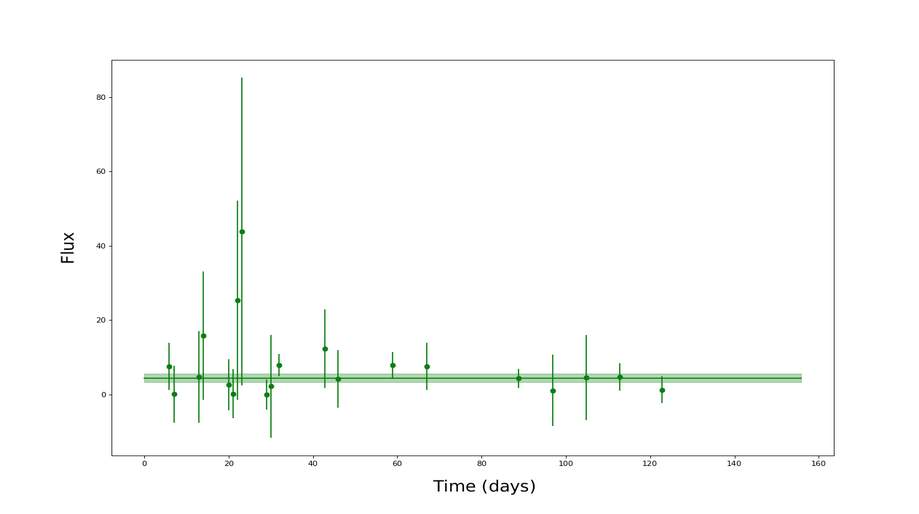
\includegraphics[width=15cm]{Ex_reta.png}
		\caption{Exemplo da interpolação não condizente com a realidade.}
		\label{fig:ExReto}
	\end{figure}
	
	\section{Delimitação}
	
	Todos os dados utilizados tanto neste trabalho quanto no artigo \cite{lochner}, foram extraídos da base de dados oferecida pelo desafio \citet{challenge}. A base de dados é de domínio público e pode ser obtida no {LINK DO DOWNLOAD}.
	
	Devido a granularidade dos dados brutos, é necessário um pré-tratamento visando buscar apenas os dados que iremos utilizar. Esse pré-tratamento foi aproveitado do \textit{pipeline} do Instituto de Física da UFRJ (\textbf{IF-UFRJ}), cujo processo visa ler os arquivos de texto transformando cada informação em uma chave de dicionário. 
	
	Ao fim do uso da seleção de dados citada acima, obtivemos valores em forma de dicionários em Python para cada objeto astronômico. Esses dicionários serão os \textbf{Dados Brutos} no escopo deste trabalho.   
	
	\section{Objetivos}
	\label{sec:Obj}
	
	O objetivo do trabalho é otimizar determinados pontos do \textit{pipeline} utilizado atualmente, após um estudo inicial ter sido feito para identificar pontos frágeis ou passíveis de melhoras.
	
	Esses pontos são apresentados e justificados a seguir, criando as três vertentes do trabalho
	
	\begin{itemize}
		\item Processo Gaussiano
		\item Aprendizagem Profunda
		\item Tratamento de \textit{Outliers}		
	\end{itemize}
	
		\subsection{Processo Gaussiano \textit{Gaussian Process}}
		
		O Processo Gaussiano, é a primeira parte do tratamento de dados após a transformação dos dados brutos em dicionários de Python. Iremos abordar esse procedimento no \autoref{chap:GP}.
		
		Cada objeto astronômico irá possuir uma quantidade de pontos que representam a intensidade do fluxo de luz captado em determinado dia, bem como a incerteza desse valor. Assim, buscamos fazer uma interpolação para obter um gráfico que passe por determinados pontos. 
		
		O objetivo ao abordar esse ponto é consertar interpolações que não condizem com a interpretação física, como pode ser vista na figura \ref{fig:ExReto}.
		
		\subsection{Aprendizagem Profunda}		

		A Aprendizagem Profunda (\textit{Deep Learning} ou \textbf{DL}) vêm sendo um advento utilizado recentemente para aprimorar alguns algoritmos de Aprendizagem de Máquina (\textit{Machine Learning} ou \textbf{ML}). 
		
		A ideia de aplicar DL nesse problema veio a partir da análise do \textit{pipeline} inicial (visto na seção \ref{sec:prob}). Tendo em vista que o mesmo possui diversas partes entre os dados brutos e algoritmo de RF, buscamos aplicar DL esperando obter um \textit{pipeline} mais simples, possuindo apenas uma etapa entre os dados brutos e o algoritmo de classificação.
		
		Em diversos outros casos na literatura, como identificação de sons ou imagens, houveram melhorias significativas ao reduzir o número de etapas envolvendo processamento de sinais (wavelets) ou redução de componentes (PCA) em troca do uso de DL. 
		
		A segunda motivação para a aplicação de DL veio do artigo da \citet{lochner}, onde ela menciona possíveis aplicações no escopo do problema.
		
		Assim, foi decidido aplicar algoritmos de DL após a primeira parte do tratamento de dados, visando manter uma simplicidade ao longo do \textit{pipeline}. Estabelecendo assim, apenas a etapa do GP entre os dados brutos e o algoritmo de classificação. O detalhamento desse procedimento encontra-se no \autoref{chap:DL}.

		\subsection{Tratamento de \textit{Outliers}}
		
		O último objetivo para buscar melhorias no algoritmo é o tratamento de pontos cuja incerteza é muito alta ou cujos valores são fora do esperado, pontos com essas características são conhecidos na literatura como \textit{outliers}.
		
		Analisando alguns dados brutos, observamos pontos cuja incerteza mostra-se mais de 100\% maior do que a própria curva (ponto mais a esquerda da figura \ref{fig:ExOutlierStd}) e também pontos que encontram-se completamente fora da curva interpolada \ref{fig:ExOutlier}.
		
		As etapas do tratamento encontram-se descritas no \autoref{chap:Out}.
		
		\newpage
		
		\begin{figure}[h!]
			\centering
			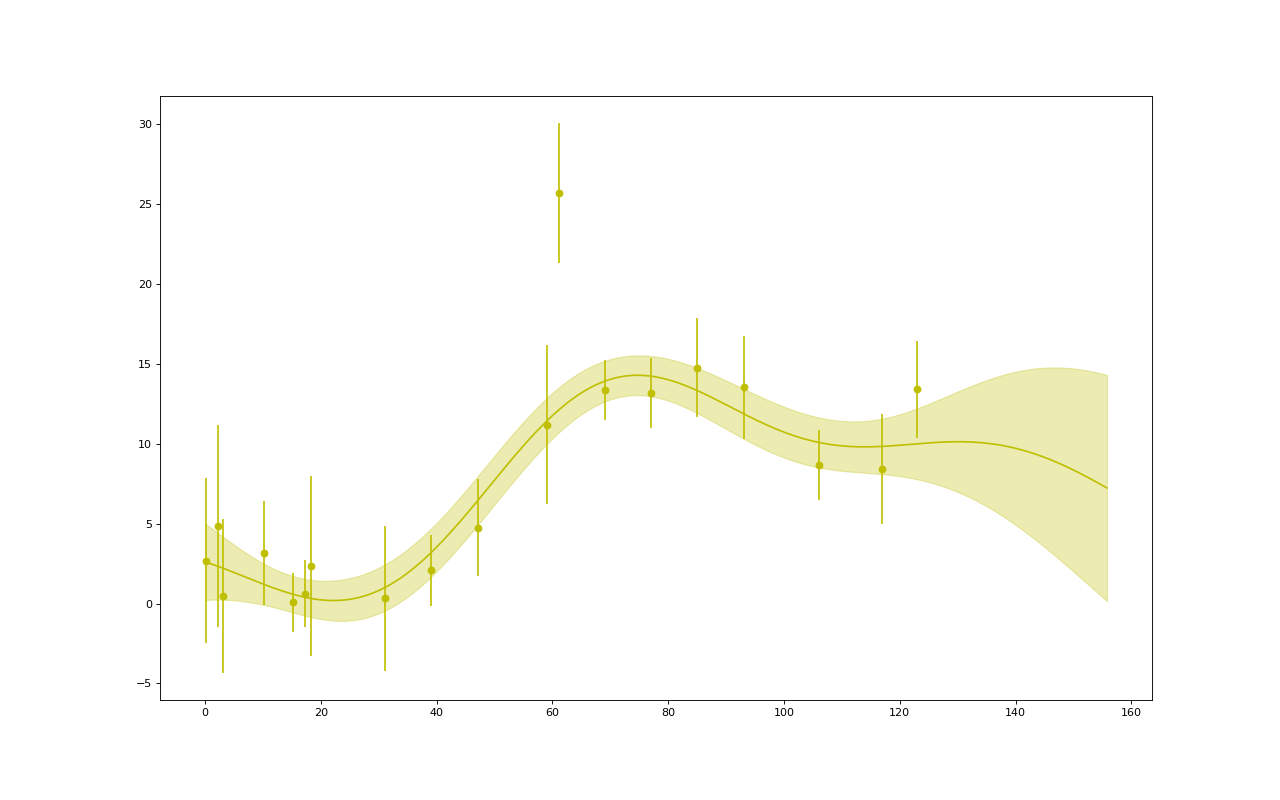
\includegraphics[width=15cm]{OutPoint.png}
			\caption[Exemplo de \textit{outlier}.]
			{{\small Exemplo de \textit{outlier}. Gráfico Fluxo $ \times $ Tempo (dias).}}
			\label{fig:ExOutlier}
		\end{figure}
	
		\begin{figure}[h!]
		\centering
		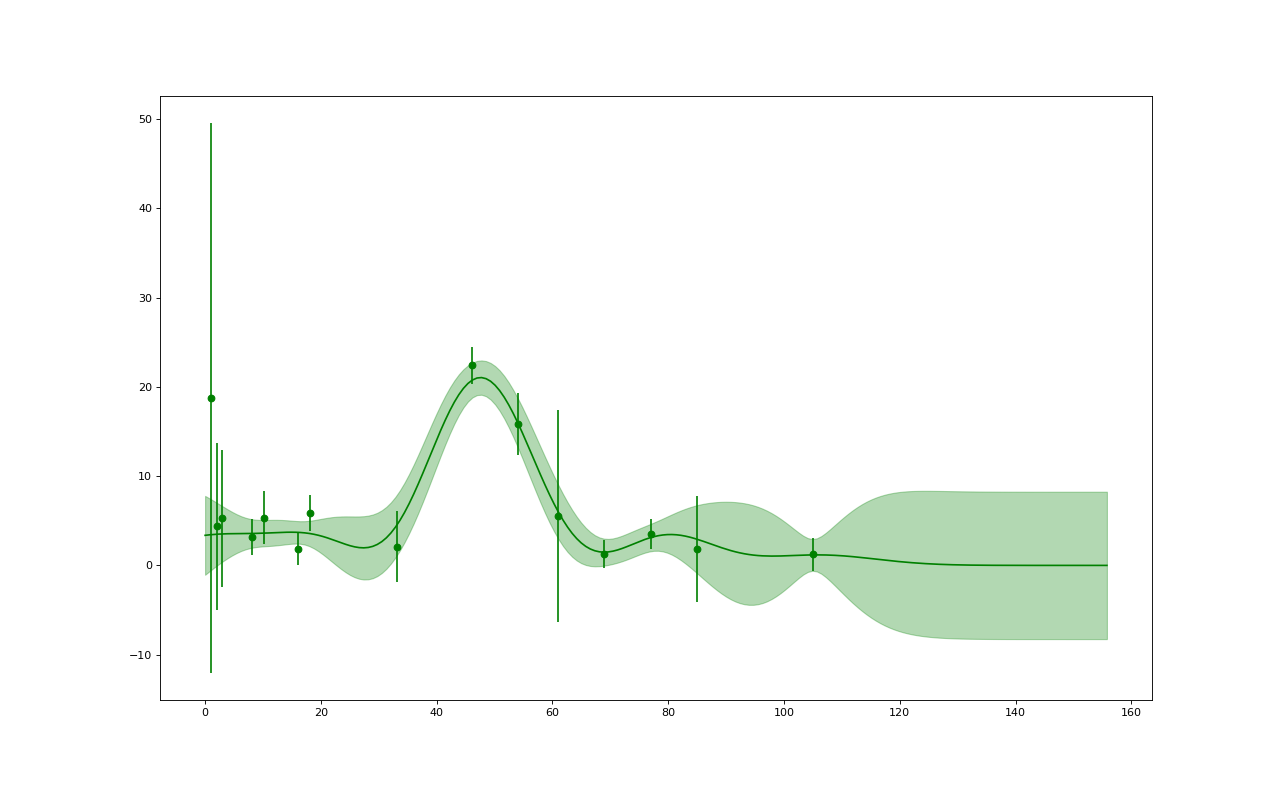
\includegraphics[width=15cm]{OutStd.png}
		\caption[Exemplo de ponto com incerteza 3 vezes maior que o pico da curva.]
		{{Exemplo de ponto com incerteza 3 vezes maior que o pico da curva. Gráfico Fluxo $ \times $ Tempo (dias).}}
		\label{fig:ExOutlierStd}
		\end{figure}
	

		
		\newpage

	\section{Metodologia}
	
	Devido ao código de pré-processamento do IF-UFRJ estar escrito em Python, todo o trabalho também foi escrito na mesma linguagem. Outro ponto para a escolha da linguagem foi a facilidade que a mesma possui para realizar experimentos através da plataforma \textit{Jupyter}, além da grande quantidade de bibliotecas de ciências de dados e suporte para desenvolver algoritmos de ML. 
	
	As principais bibliotecas utilizadas no contexto de tratamento de dados foram \textit{Pandas} e \textit{Numpy}. Já para a aplicação dos métodos as bibliotecas mais importantes foram \textit{scikit-learn}, \textit{Keras} e \textit{PyMC3}.
	
	A entrada dos modelos sempre serão os dicionários gerados a partir dos dados brutos após o pré-processamento do IF-UFRJ. Assim, pôde-se  filtrar com maior facilidade as propriedades desejadas para cada uma das três vertentes do trabalho. 

	Cada uma dessas vertentes possuiu um trabalho específico e isolado para poder melhor averiguar suas mudanças posteriormente. Em outras palavras, a cada mudança realizada houve a comparação direta com os resultados do \textit{pipeline} original, para poder avaliar especificamente a eficiência e melhora dessa mudança.
	
	Por se tratar de um algoritmo de classificação, a saída do nosso modelo será booleana e classificará se um objeto astronômico é ou não do tipo IA. Entretanto, nos dados brutos, as classes são divididas em 8 tipos de objetos: \textit{IA, IB, IBC, IC, II, IIL, IIN} e \textit{IIP}.
	
	É importante ressaltar também que para validar os modelos do projeto, foi usado o método \textit{K-fold}. Todavia, este trabalho se diferenciou da divisão clássica presente na literatura, que é uma divisão de 80\% dos dados para treinamento e 20\% para o teste dos modelos. Neste trabalho foram utilizados apenas 1100 objetos para treino dentre 21316 objetos totais. A justificativa é a limitação física das amostras.
	
	Por fim, as mudanças foram verificadas através de \textbf{Matrizes de Confusão} (\textit{Confusion Matrices} ou \textbf{CM}) ou através de métodos de \textit{score} da biblioteca \textit{scikit-learn}.
	
	Como última observação, a fim de estudos posteriores fora do escopo do projeto, foram feitas classificações envolvendo os 8 tipos de objetos, além de treinamentos adotando a proporção de 80\% para treino e 20\% para teste.
		
		
		
	\section{Descrição}
	No \autoref{chap:FundTeo}, iremos explicar os principais conceitos teóricos utilizados na aplicação do \textbf{Processo Gaussiano} e no \textbf{\textit{Deep Learning}}. Também serão levantados alguns conceitos não tão centrais do trabalho, mas de importância igualmente significativa.
	
	O \autoref{chap:ModeloAtual} será destinado para detalhar especificamente cada etapa do \textit{pipeline} atual, assim como uma breve menção a maneira na qual os dados brutos são tratados.
	
	Os capítulos 4, 5 e 6 serão destinados à explicação dos objetivos citados na seção \ref{sec:Obj}, assim como os resultados das mudanças que os mesmos causaram, buscando averiguar a eficiência de aplicação ou explicar possíveis erros.
	
	No \autoref{chap:Result} serão apresentados os resultados como um todo, seguidos de análises dos métodos através uma perspectiva global do projeto, diferentemente de como será nos capítulos anteriores, nos quais teremos uma visão específica para cada objetivo.
	
	Por fim, no \autoref{chap:Concl} tiraremos as conclusões finais do projeto e serão apresentadas sugestões de trabalhos futuros junto as limitações e possíveis soluções encontradas.
	
	\newpage
	
  \chapter{Fundamentos Teóricos}
  \label{chap:FundTeo}
  
 	\section{Processo Gaussiano}
 	
 	O Processo Gaussiano é uma ferramenta importante no escopo de \textit{Machine Learning} que nos permite fazer predições sobre nossos dados tendo como base um conhecimento a priori. A sua aplicação mais frequente é em interpolações de funções, vide a aplicação neste projeto. Há também possíveis aplicações do conceito em classificações e agrupamentos de grande quantidades de dados. O livro base utilizado para os estudos desse projeto foi \citet{GPBook} . 
 	
 	Sabendo que para uma quantidade determinada de pontos existe uma infinidade de funções que podem interpolar esses valores, o Processo Gaussiano realiza essa interpolação a partir dos conhecimentos a priori dos valores dessa função, assim como de um provável formato que ela pode assumir como um todo. Por fim, o GP não irá obter um valor específico para cada ponto da função interpolada, mas sim uma distribuição probabilística para cada ponto, onde cada um possuirá uma média (valor que será atribuído) e um desvio padrão (incerteza).
 	
 	Neste projeto não abrangeremos maiores detalhes para o aprendizado do método, contudo, pode-se encontrar na bibliografia, tanto referências mais específicas e técnicas \cite{GPBook},   quanto mais práticas \cite{ridge}, \cite{GPDummies}, \cite{GPVisual}.
 	
 	Iremos agora focar nos dois aspectos fundamentais do Processo Gaussiano; eles serão os principais responsáveis por caracterizar as interpolações.

	\subsection{\textit{Kernel} e Função de Covariância}
	
	O Processo Gaussiano interpola uma função discreta de $n$ pontos através dos $m$ pontos conhecidos, resultando em $n$ distribuições normais, uma para cada ponto que irá constituir essa função discreta.
	
	Vale lembrar que uma função discreta cujos intervalos dos pontos do eixo das abscissas são significativamente pequenos pode ser considerada contínua para efeitos práticos. 
	
	O diferencial do GP é considerar uma distribuição normal multivariável de dimensão $n+m$ durante a interpolação. Essa distribuição normal multivariável possuirá uma covariância $\Sigma$ responsável não apenas por descrever o \textbf{formato}, como também por determinar \textbf{características} da função a ser prevista.
	
	Para poder obter o $\Sigma$ desta normal multivariável, é estabelecido o \textit{Kernel} do GP. Ele é uma função de duas variáveis especial que respeita certas restrições matemáticas (Cap. 4 \citet{GPBook}). Essas varíaveis são os valores da abscissa de cada ponto da função a ser interpolada.
	
	Em outras palavras, o \textit{Kernel} é uma função que irá relacionar dois pontos que deverão estar na curva interpolada, baseando se apenas na distância entre eles. É essa relação que fornecerá características como periodicidade, picos e suavização da curva.
	
	É importante ressaltar que apenas os valores das abscissas serão utilizados para essa relação, enquanto os valores das ordenadas dos pontos conhecidos são utilizados para forçar que essa função passe pelos pontos dados, através de \textbf{probabilidade condicionada} ( \textit{\textbf{Posterior Distribution}} \cite{GPVisual}). Pode-se utilizar esse método de probabilidade condicionada devido à propriedade das distribuições gaussianas que afirma: distribuições condicionadas ou marginalizadas vindas de distribuições gaussianas também são gaussianas. 
	
	A figura \ref{fig:Kernel} ilustra uma maneira mais fácil de visualizar o que foi dito no parágrafo acima. Pode-se ver em \ref{fig:Kernel}(b) que os mesmos 10 pontos serão calculados já com a probabilidade condicionada para satisfazer os 2 pontos pré-estabelecidos.
	
	\begin{figure*}
		\centering
		\begin{subfigure}[h]{0.475\textwidth}
			\centering
			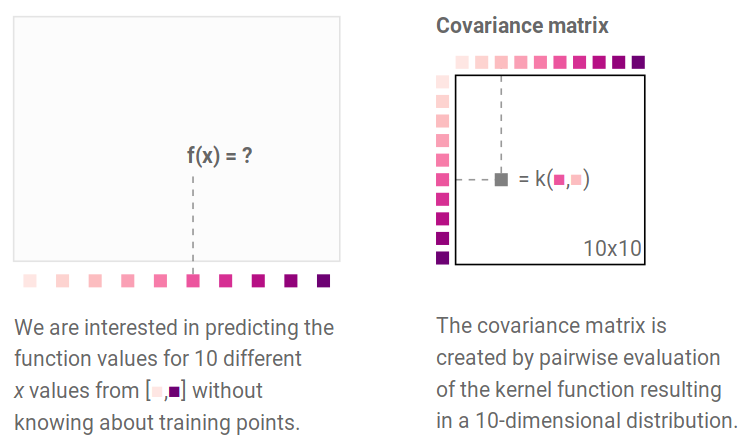
\includegraphics[width=1.1\textwidth]{Kernel1.png}
			\caption[]%
			{{\small Ilustração da matriz $\Sigma$ para 10 pontos.}}    
			\label{fig:Kernel1}
		\end{subfigure}
		\vskip\baselineskip
		\begin{subfigure}[h]{0.475\textwidth}   
			\centering 
			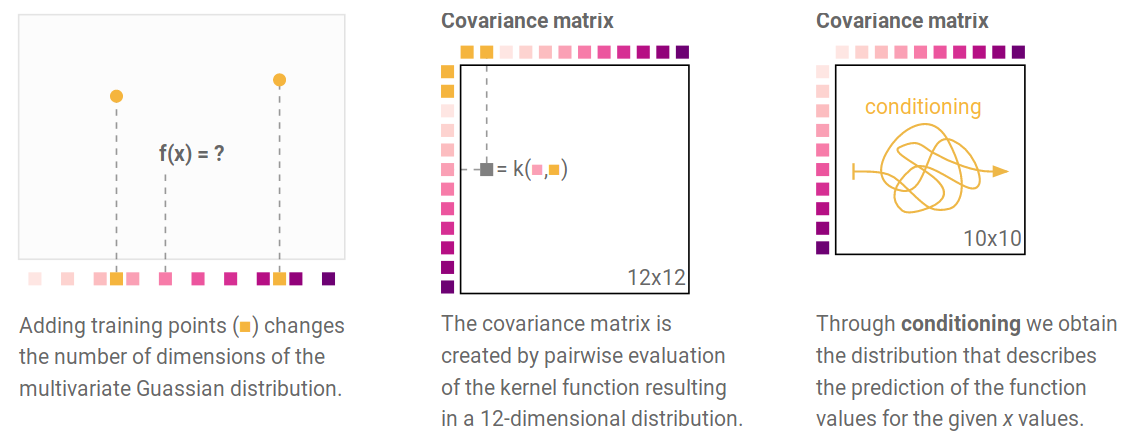
\includegraphics[width=1.1\textwidth]{Kernel2.png}
			\caption[]%
			{{\small Ilustração da matriz $\Sigma$ para 12 pontos. 2 deles são pontos dados.}}    
			\label{fig:Kernel2}
		\end{subfigure}
		\quad

		\caption[ Ilustração da matriz $\Sigma$ possuindo 10 e 12 pontos.]
		{\small Ilustração da matriz $\Sigma$ possuindo 10 e 12 pontos. \textit{Imagens retiradas de \citet{GPVisual}}} 
		\label{fig:Kernel}
	\end{figure*}
	
	\newpage
 	
 	\subsection{Função Média}
 	
 	A Função Média de um Processo Gaussiano é aquela responsável por oferecer a predição inicial do ponto a ser interpolado. É o valor que determinado ponto possuiria caso só existisse ele a ser definido.
 	
 	Contudo, só existe sentido em falar de função média caso a associemos à Função Covariância. Normalmente a Função Média é estabelecida como uma distribuição normal com média em 0 e desvio padrão 1. 
 	
 	É possível usar essa distribuição padrão como valor a priori, pois o valor final da média de um ponto será obtido após um número suficientemente grande de amostras de pontos, que serão definidos através de amostragens usando \textbf{Cadeias de Markov Monte Carlo} \cite{MCMC}, se aproximando cada vez mais do valor ideal. A figura \ref{fig:MCMC}(a) ilustra esse caso.
 	
 	Todavia, é imprescindível o uso correto da Função Média, pois caso ela tenha seu domínio delimitado, isso poderá impossibilitar que a função assuma alguns valores, como está ilustrado na \ref{fig:MCMC}(b).
 	
 	\begin{figure*}
 		\centering
 		\begin{subfigure}[h]{0.475\textwidth}
 			\centering
 			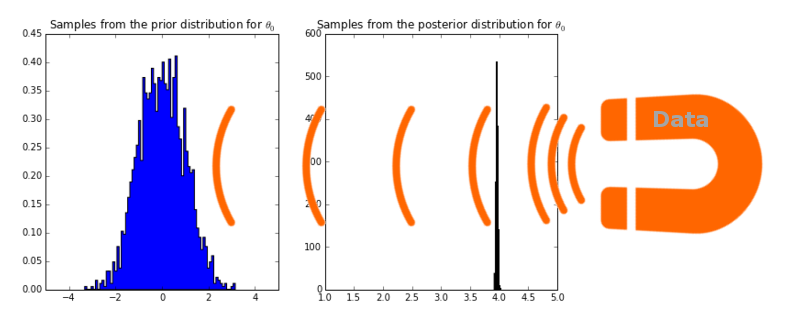
\includegraphics[width=1.1\textwidth]{mcmc1.png}
 			\caption[]%
 			{{\small Exemplo de priori gaussiana que ao longo das amostragens influenciadas pelos dados assume o valor real (no caso do exemplo é 4).}}    
 			\label{fig:MCMC1}
 		\end{subfigure}
 		\vskip\baselineskip
 		\begin{subfigure}[h]{0.475\textwidth}   
 			\centering 
 			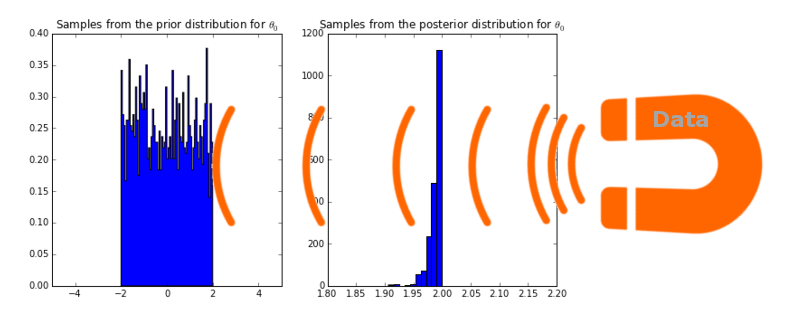
\includegraphics[width=1.1\textwidth]{mcmc2.png}
 			\caption[]%
 			{{\small Exemplo de priori delimitada que mesmo ao longo das amostragens nunca assumirá o valor real (no caso do exemplo é 4 e a delimitação é de -2 a 2).}}    
 			\label{fig:MCMC2}
 		\end{subfigure}
 		\quad
 		
 		\caption[ Ilustração do valor da função média.]
 		{\small Ilustração do valor da função média durante as amostragens via Cadeias de Markov Monte Carlo. \textit{Imagens retiradas da \citet{GPDummies}} } 
 		\label{fig:MCMC}
 	\end{figure*}
 	

 	
 	\section{Convolutional Neural Network}
 	\label{sec:CNN}
 	
 	Convolutional Neural Network (\textbf{CNN}) is a part of Deep Learning (\textbf{DL}) which is most commonly applied to analyze visual data. Our main goal inside this project is to use Machine Learning algorithms, however, to avoid any ambiguity with the nomenclatures, it is important to say that Deep Learning is a part of a broader Machine Learning family.
 	
 	A basic DL architecture is made by 3 parts (figure \ref{fig:DLArch}):
 	
 	\begin{itemize}
 		\item Input Layer: The first layer, being responsible for receiving one data sample and passing it to the hidden layers. 
 		\item Hidden Layers: The internal DL architecture structure, inside this part are set and trained the functions to process and classify the data.
 		\item Output Layer: The last Layer. It will be responsible for the final answer. In this project it will have the values of 0 and 1, respectively for classified supernovas as \textit{non IA} and \textit{IA}.
 	\end{itemize}
 	
 	Each layer is composed by different types of \textbf{neurons}. Those neurons are mathematical functions with specific parameters, which will be trained in order to classify our data.
 	
 	\begin{figure}[h!]
 		\centering
 		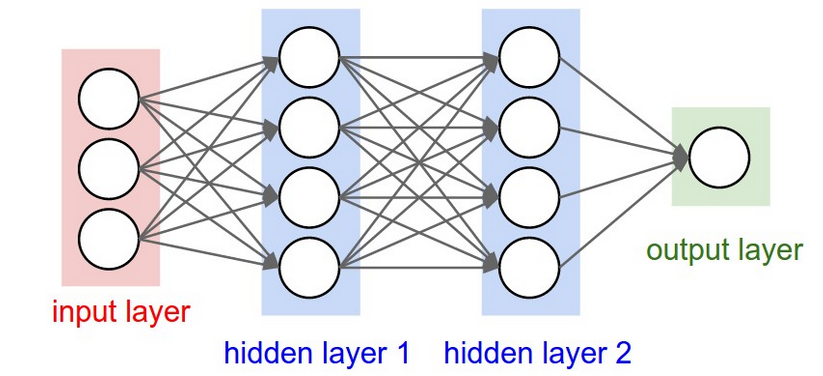
\includegraphics[width=12cm]{DLarch.png}
 		\caption[Deep Learning Standard Architecture.]
 		{{Deep Learning Standard Architecture. (adapted from: \href{https://en.proft.me/2016/06/15/getting-started-deep-learning-r/}{here}.)}}
 		\label{fig:DLArch}
 	\end{figure}
 	
 	In this project it is used CNN, a specific type of mathematical procedure compounding the hidden layer normally designed to process images. This thesis uses black and white png files created from a Gaussian Process interpolation.
 	
 	Firstly, the CNN must receive the image in a matrix format, where each pixel is a value between 0 and 1 (0 for white and 1 for black varying through gray's intensities). Therefore, the hidden layers process the matrices using different methods \ref{fig:convolution}(e.g. max pooling, ordinary convolution).

 	\begin{figure}[h!]
		\centering
		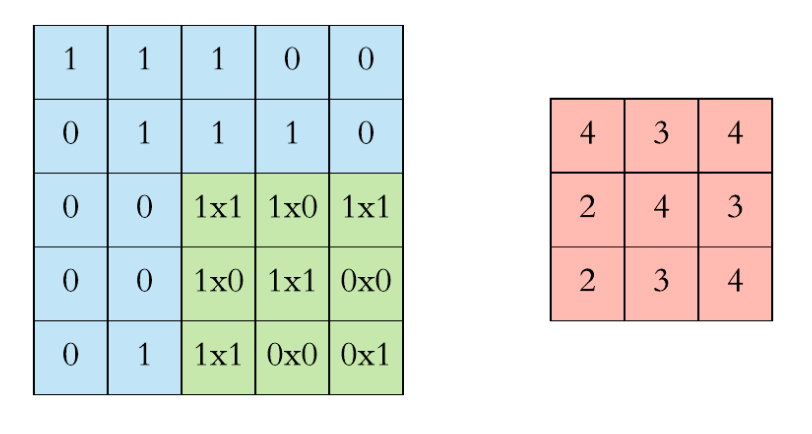
\includegraphics[width=12cm]{convolution.png}
		\caption[Convolution Operation.]
		{{The blue matrix represents the input values; the red one is the result of convolution operation; and the green matrix contains the parameters to multiply the values from the blue one "sliding through its grid". (adapted from: \href{https://towardsdatascience.com/applied-deep-learning-part-4-convolutional-neural-networks-584bc134c1e2}{here}.)}}
		\label{fig:convolution}
	\end{figure}
 	
 	Through different possible existent CNN methods, there is one particular which was used inside this project. It is the Max pooling. It consists on taking the biggest value after a matrix convolution \ref{fig:maxpooling}. 
 	
 	\begin{figure}[h!]
 		\centering
 		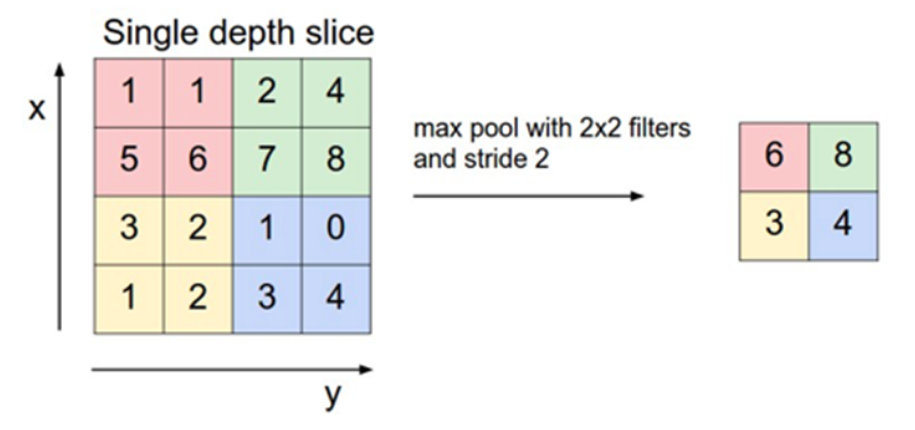
\includegraphics[width=12cm]{maxpooling.png}
 		\caption[Max Pooling.]
 		{{Max pooling example, it selects the biggest value of a specific matrix and reduces the dimension of it only filtering that value. (adapted from: \href{http://cs231n.github.io/convolutional-networks/\#pool}{here}.)}}
 		\label{fig:maxpooling}
 	\end{figure}
 	
 	Inside the hidden layers it is impossible to say exactly what is the physical meaning of each of them. Some might be nothing but mathematical function results converging to a final classification. But sometimes it is still possible to identify one layer as an image property like edges, eyes, foots, curves, etc.
 	
 	Finally, with those techniques of evaluating and processing images, the last layer will receive the results from the hidden ones and returns a value responsible for the classification (mostly like numbers).
 	
 	It is important to mention that there is a little randomness inside this process of training and optimizing the internal layers' parameters.
  
 	\section{Demais Conceitos}
 	\label{sec:OtherConcepts}
 	
 	Aqui estão apresentados alguns conceitos menos usados ao longo do \textit{pipeline}.
 		
 		\subsection{Análise de Componentes Principais}
 		
 		A Análise de Componentes Principais (Cap. 12 \citet{ML}), ou \textit{Principal Component Analysis} (\textbf{PCA}), utiliza conceitos de ortogonalizações de vetores para poder reduzir dimensões.
 		
 		Em ML, essa redução de dimensões é aplicada as \textit{features} de um \textit{dataframe}, onde as amostras possuem um grande número de características e deseja-se reduzi-las para que o modelo de aprendizagem de máquina seja menos pesado mas igualmente eficaz.
 		
 		Através de técnicas vindas da álgebra linear o método "cria" novas dimensões virtuais compostas por combinações lineares das existentes, de maneira que estas novas dimensões poderão melhor distinguir a quantidade de dados existentes no \textit{dataframe}. 
 		
 		Por fim pode-se também interpretar PCA por uma perspectiva de filtros, onde se decompõe determinado sinal, e selecionando determinadas frequências conserva-se a potência do sinal. Por esta perspectiva, as frequências são as \textit{features} e a potência é a porcentagem que as novas \textit{features} têm de representar o \textit{dataframe}.
 		
 		\subsection{Transformadas de \textit{Wavelet}}
 		
 		Transformadas de \textit{Wavelet} \cite{Afonso} ou onduletas são funções capazes de descrever ou representar outras funções em diferentes escalas de frequência e de tempo.
 		
 		São normalmente usadas no domínio de processamento de sinais, sendo úteis para eliminar ruídos e comprimir dados por exemplo.
 		
 		Neste projeto as Transformadas de \textit{Wavelet} servem para processar os gráficos interpolados do GP. Resultando assim em valores que podem ter possíveis erros de interpolação eliminados, por exemplo. 
 		
  		\subsection{K-Fold Cross Validation}
  		
  		Cross-validation is a family of statistical methods used to estimate how a model can be generalized regardless the train and test sets.
  		
  		In ML, it is commonly used to analyze if a model is robust enough or if it gives more false-positives and false-negatives (inside the classification cases).
  		
  		K-Fold Cross Validation is one of these methods. The procedure consists in dividing the data set in $K$ folds, \textbf{normally} $K-1$ are used to train the model while $1$ is used to test.  However in this project, due to physical limitation reasons only 1 fold is used to train while the other 18 are used to test and validate the method (the value of K is set to be 19).
  		
  		With the K-Fold idea there are 2 concepts which will be used to evaluate the results in this project:
  		
  		\begin{itemize}
  			\item AUC Curve (Cap. 5.7 \citet{ML})
  			\item Mean Average Precision (Cap. 9.7.4 \citet{ML})
  		\end{itemize}
  	
  		 
  		
	\newpage
  \chapter{Modelo Atual}
  \label{chap:ModeloAtual}  		
  
  Neste capítulo iremos detalhar o modelo atual utilizado para estudos cosmológicos do IF-UFRJ.


	\section{Pré-processamento dos Dados Brutos}
	
	Como pode ser visto na figura \ref{fig:RawData}, os dados brutos chegam da seguinte forma para o pré-processamento.
	
	
	\begin{figure}[ht]
		\centering
		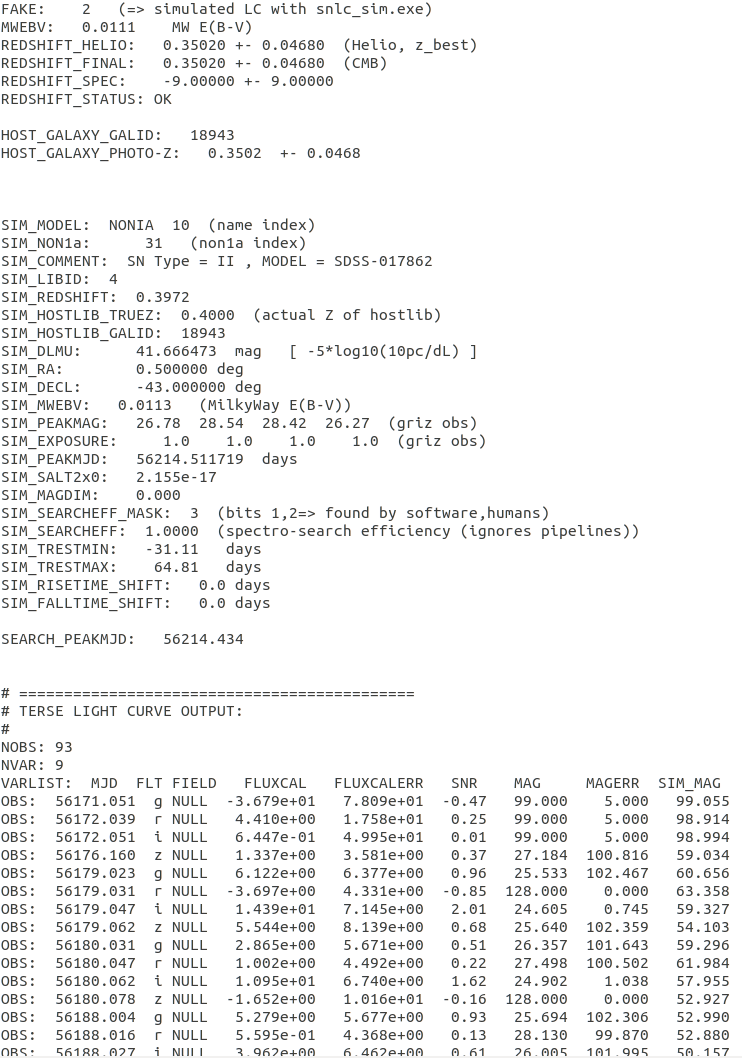
\includegraphics[width=9cm]{raw_dat.png}
		\caption{Arquivo \textit{.txt} a ser lido pelos arquivos de pré-processamento.}
		\label{fig:RawData}
	\end{figure}
	
	Através dos arquivos de pré-tratamento iremos obter todas essas informações em forma de dicionário, entretanto apenas as seguintes serão utilizadas durante o projeto.
	
	\begin{itemize}
		\item \textbf{SN TYPE} : Informa o tipo de supernova
		\item  \textbf{TERSE LIGHT CURVE OUTPUT} : Informa os pontos de observações obtidos. Será nosso \textit{Data Frame}. 
		\begin{itemize}
			\item \textbf{MJD} : O momento em que a observação foi obtida. A medida está descrita em dias do calendário Juliano.
			\item \textbf{FLT} : O filtro em que a observação foi obtida, pois cada observação é obtida a partir de um determinado espectro de luz. 
			\item  \textbf{FLUXCAL} : O valor do fluxo de luz obtido naquela observação.
			\item  \textbf{FLUXCALERR} : O valor do erro do fluxo de luz obtido naquela observação.
		\end{itemize}
	\end{itemize}

	Em relação ao \textbf{MJD}, vale ressaltar que é um método usado na astronomia para contar os dias sequencialmente, começando em uma data arbitrária no passado. Neste projeto, essas datas serão normalizadas, tendo como 0 o menor valor do MJD para que nosso eixo das abscissas tenha sempre início em 0.

	Em relação ao \textbf{FLT}, cada objeto astronômico é visto através de 4 filtros de luz diferentes, obtendo assim 4 curvas de luz para cada um deles. Para efeitos de aprendizagem de máquina, cada objeto possuirá 4 \textit{data frames}, um para cada filtro, e posteriormente essas propriedades serão convertidas em \textit{features} de cada objeto.
	
	A figura \ref{fig:ExFiltro} ilustra as 4 curvas de luz para o mesmo objeto.
	
	\begin{figure*}
		\centering
		\begin{subfigure}[b]{0.475\textwidth}
			\centering
			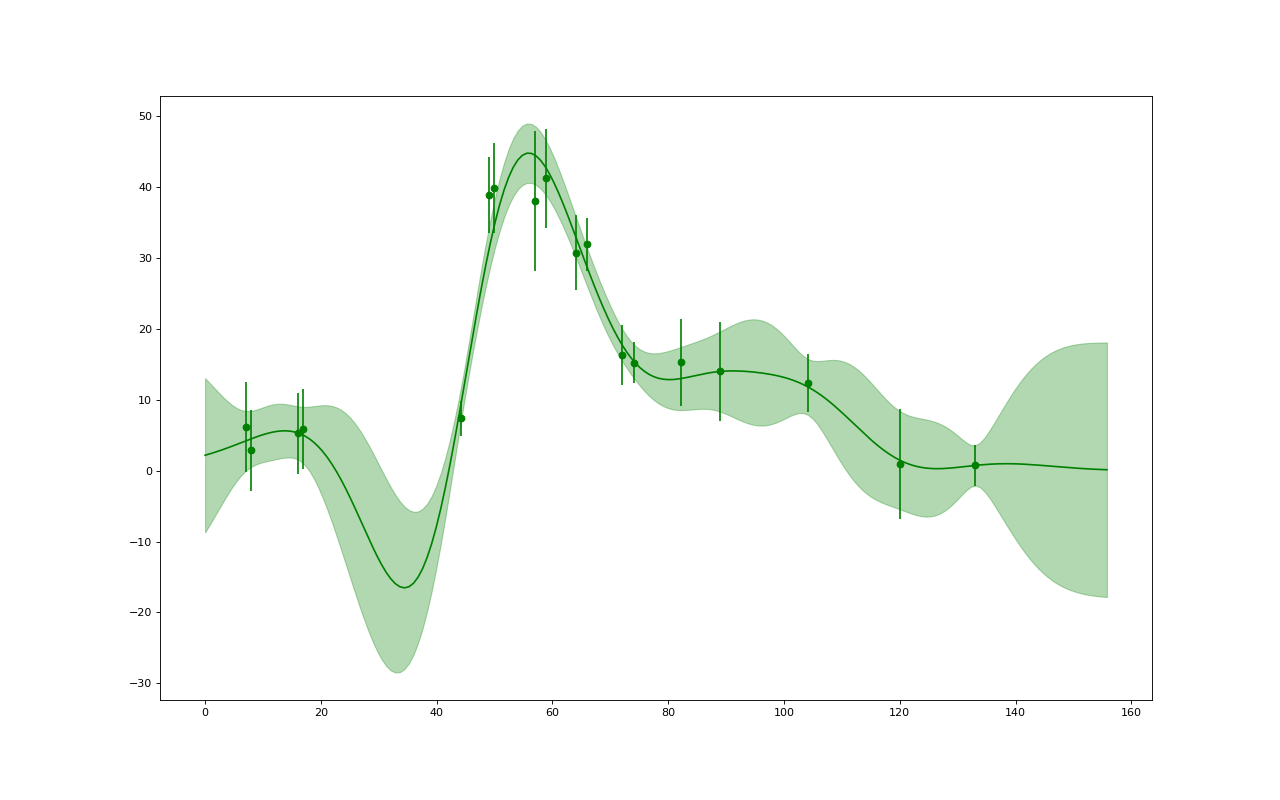
\includegraphics[width=\textwidth]{SN000017_II_desg.png}
			\caption[]%
			{{\small Filtro \textit{desg}}}    
			\label{fig:mean and std of net14}
		\end{subfigure}
		\hfill
		\begin{subfigure}[b]{0.475\textwidth}  
			\centering 
			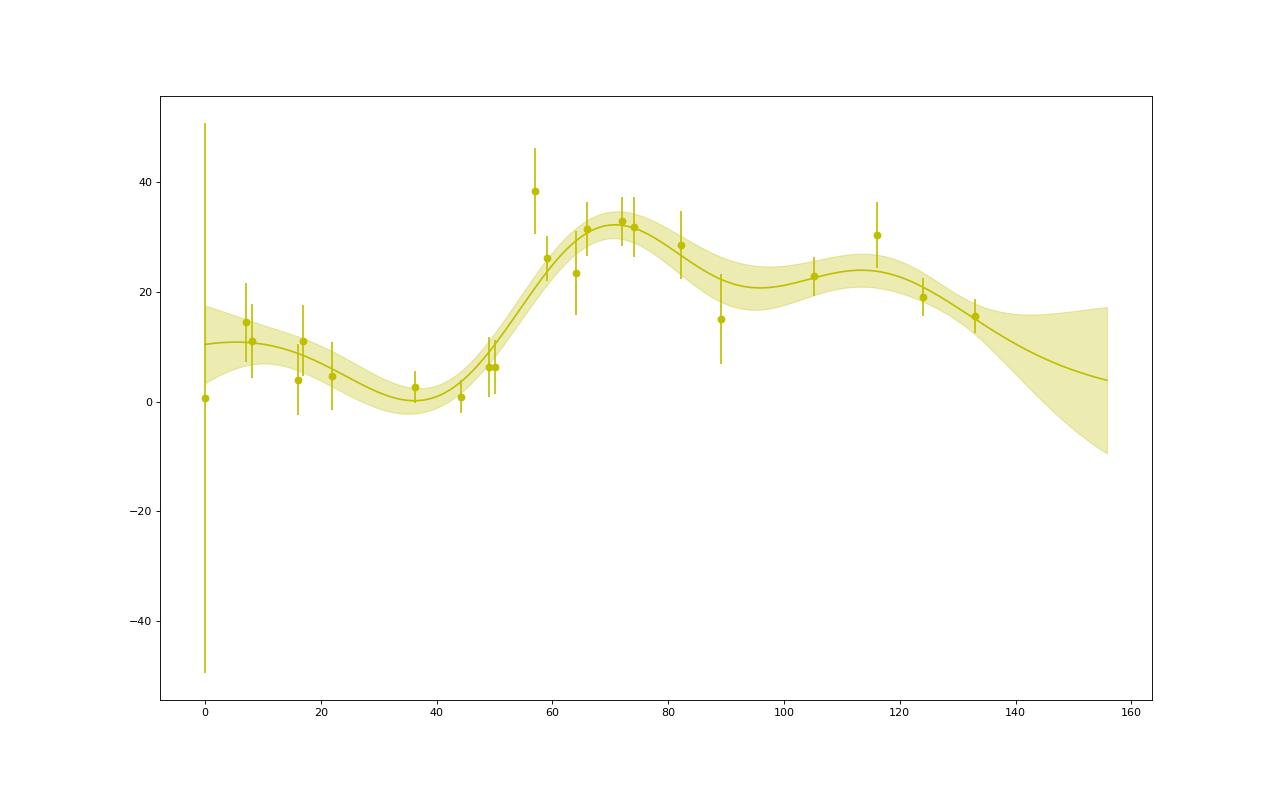
\includegraphics[width=\textwidth]{SN000017_II_desi.png}
			\caption[]%
			{{\small Filtro \textit{desi}}}    
			\label{fig:mean and std of net24}
		\end{subfigure}
		\vskip\baselineskip
		\begin{subfigure}[b]{0.475\textwidth}   
			\centering 
			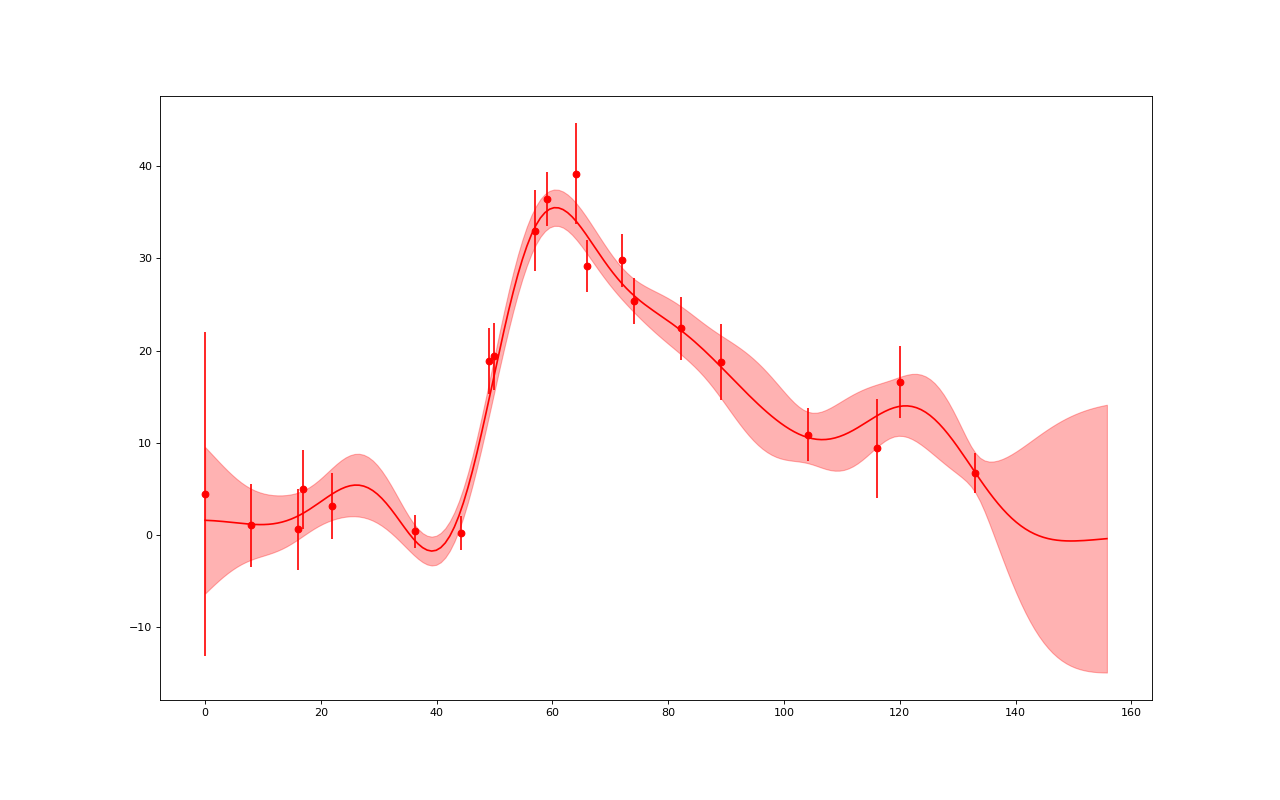
\includegraphics[width=\textwidth]{SN000017_II_desr.png}
			\caption[]%
			{{\small Filtro \textit{desr}}}    
			\label{fig:mean and std of net34}
		\end{subfigure}
		\quad
		\begin{subfigure}[b]{0.475\textwidth}   
			\centering 
			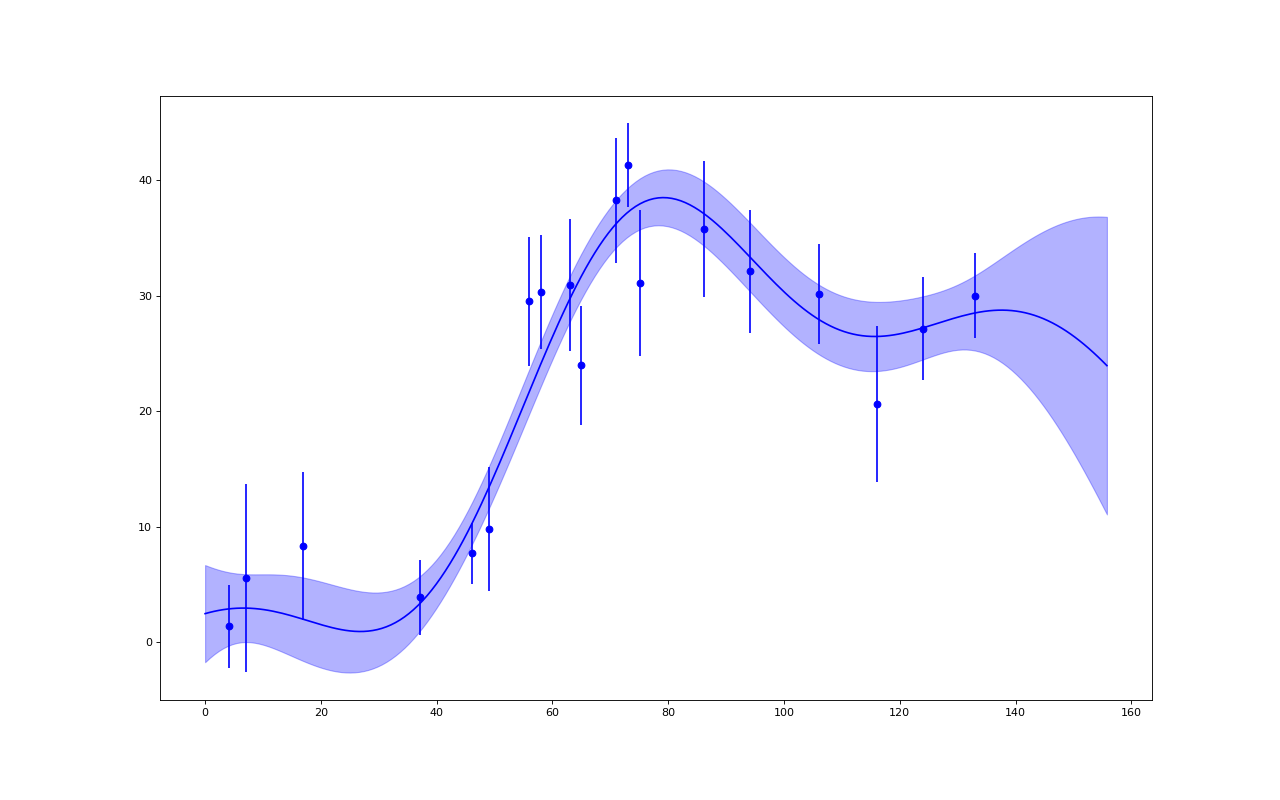
\includegraphics[width=\textwidth]{SN000017_II_desz.png}
			\caption[]%
			{{\small Filtro \textit{desz}}}    
			\label{fig:mean and std of net44}
		\end{subfigure}
		\caption[ Exemplo de 4 curvas de luz de um mesmo objeto.]
		{\small Exemplo de 4 curvas de luz de um mesmo objeto, uma para cada filtro. Gráfico Fluxo $ \times $ Tempo (dias).} 
		\label{fig:ExFiltro}
	\end{figure*}
	
	\section{\textit{Pipeline} Atual}
	
	A partir do pré-processamento explicado na seção anterior, o \textit{pipeline} atual irá dispor destes dados para realizar as etapas do processo de classificação.
	
	Inicialmente ele irá separar os dados do \textit{Terse Light Curve Output} pelos filtros e irá criar 4 \textit{numpy arrays} possuindo $n \times 3$ dimensões cada (\textbf{MJD}, \textbf{FLUXCAL} e \textbf{FLUXCALERR}) e sendo n o número de amostras.
	
	Em seguida, esses 4 \textit{numpy arrays} serão a entrada do modelo de \textit{Gaussian Process}, cuja função é interpolar uma curva que passe pelos pontos de cada filtro, como pode ser visto na figura \ref{fig:ExFiltro}.
	
	A saída do Processo Gaussiano será o gráfico interpolado em forma de \textit{numpy array} $100 \times 3$, contendo 100 pontos de abscissa, 100 pontos de ordenada e 100 pontos do erro da ordenada. 
	
	Essa saída será a entrada do processo de \textit{wavelets}, que irá retornar 400 valores para cada entrada. 
	
	No total, cada objeto terá esse procedimento feito 4 vezes, uma para cada filtro. Assim, como saída do processo de \textit{wavelets} teremos 1600 coeficientes para cada objeto astronômico.
	
	Em seguida, é realizada uma redução de variáveis através da \textbf{análise de componentes principais} ou \textbf{PCA}. Após esse procedimento, cada objeto possuirá 20 \textit{features}.
	
	Após essa etapa, o \textit{dataframe} já estará composto por 21316 amostras com 20 \textit{features} cada.
	
	Em paralelo, usamos o \textbf{SN TYPE} do dicionário para guardar os \textit{labels} de cada objeto astronômico em forma de lista.
	
	Finalmente será criado o modelo de classificação baseado em \textit{Random Forest} para classificar o tipo de objeto astronômico. Usamos o módulo \textit{sklearn.pipeline} da biblioteca \textit{scikit learn}.
	
	Tendo em mãos o \textit{dataframe}, a lista com as classificações de cada objeto (os \textit{labels}) e o modelo de classificação, é feito a divisão usando o método \textit{k-fold} de validação cruzada. Nele dividimos os objetos em 19 partições e usa-se 1 delas para treino e as demais para teste.
	
	Por fim, cada modelo dos 19 \textit{folds} existentes é avaliado através de 2 maneiras de obtenção de \textit{score}, a \textbf{curva AUC} e o \textbf{método de precisão média} (seção \ref{sec:OtherConcepts}). Podemos também analisar as matrizes de confusão de cada um dos 19 modelos para ilustrar seus acertos, seus falsos positivos e falsos negativos (figura \ref{fig:CMEx}). 

	\begin{figure*}[h]
	\centering
	\begin{subfigure}[b]{0.475\textwidth}
		\centering
		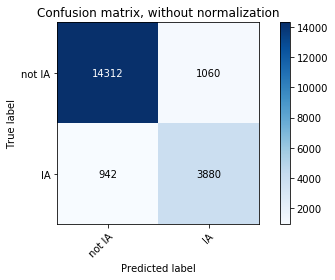
\includegraphics[width=\textwidth]{cm_ex.png}
		\caption[]%
		{{\small Exemplo de Matriz de Confusão, valores absolutos.}}    
		\label{fig:CMExValor}
	\end{subfigure}
	\hfill
	\begin{subfigure}[b]{0.475\textwidth}  
		\centering 
		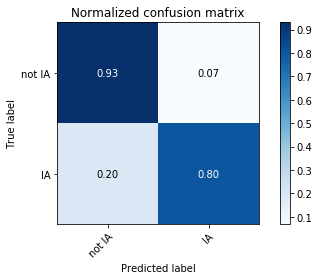
\includegraphics[width=\textwidth]{cm_exp.png}
		\caption[]%
		{{\small Exemplo Matriz de Confusão, valores normalizados.}}    
		\label{fig:CMExPorcentavem}
	\end{subfigure}
	\caption[ Exemplo de Matrizes de Confusão de um modelo final do \textit{pipeline} original. ]
	{\small Exemplo de Matrizes de Confusão de um modelo final do \textit{pipeline} original.} 
	\label{fig:CMEx}
	\end{figure*}
	
	\newpage
  \chapter{Tratamento de \textit{Outliers}}
  \label{chap:Out}
 	
 	\section{Estratégias Utilizadas}  	
 	
 	
 		
 	\section{Resultados e comparações}
	\newpage 		
  \chapter{Rede Neural Convolucional}
  \label{chap:DL}
 	A abordagem utilizando \textit{Deep Learning} embasou-se em uma breve análise dos dados onde se percebeu algumas diferenças entre gráficos de diferentes tipos de objetos astronômicos, assim como pequenas semelhanças entre aqueles do mesmo tipo.
 	
 	Somou-se a isso o conhecimento vindo da literatura de que recentemente muitos algoritmos rebuscados com diversas etapas em seu \textit{pipeline} vêem sendo substituídos por \textit{pipelines} mais simples contendo \textit{Deep Learning}.
 	
 	 \section{Geração de Imagens e Parâmetros}  
 	 
 	 A primeira etapa desta abordagem consiste em gerar gráficos a partir da interpolação gaussiana. Vale lembrar que para comparar o resultado deste método com o \textit{pipeline} inicial, a interpolação realizada para gerar os gráficos fornecidos ao DL é a mesma interpolação usada no \textit{pipeline} original.
 	 
 	 Optou-se gerar gráficos ao invés de utilizar os pontos diretamente, devido à interpolação possuir mais informações ao aprendizado da máquina do que apenas pontos soltos em uma imagem. 
 	 
 	 Estas imagens serão gráficos em escalas de cinza na extensão \textit{png} cujas dimensões são:$64 \times 40$ pixels. Ao analisá-las, notou-se que existe uma margem ao gerar as imagens, esta margem contém 5 pixels na dimensão $y$ e 9 pixels na dimensão $x$. Para otimizar o tempo de treinamento, após transformar as imagens em matrizes \textit{numpy} eliminaram-se também essas margens, resultando em um formato de dimensão $46 \times 30$.
 	 
 	 Por fim, vale ressaltar que essas dimensões foram escolhidas baseando-se em exemplos clássicos e bem conhecidos da literatura que possuem dimensões com valores bem próximos, como o \href{	https://towardsdatascience.com/image-classification-in-10-minutes-with-mnist-dataset-54c35b77a38d
 	 }{MNIST} e \href{https://github.com/zalandoresearch/fashion-mnist}{Fashion MNIST}.

 	\section{\textit{Pipeline}}  	
 	
 	Após a transformação dos arquivos de imagem para matrizes de \textit{nparray}, foi construída uma estrutura de dados para cada objeto como um compilado de suas 4 figuras. Obtendo o formato final de \textbf{(21316, 4, 30, 46)}, onde:
 	\begin{itemize}
 		\item Número de objetos: 21316
		\item Número de imagens ou matrizes (referente a cada filtro): 4
		\item Número de pixels por coluna (ou número de linhas): 30
		\item Número de pixels por linha (ou número de colunas): 46   
		
 	\end{itemize}
 
 	Dentre diversos possíveis tipos de camadas internas de \textit{Deep Learning} foram escolhidas camadas do tipo \textbf{Convolucionais 2D} e \textbf{\textit{Max Pooling} 2D} (seção \ref{sec:CNN}).
 	
 	A arquitetura escolhida também foi baseada em exemplos clássicos de problemas de identificação de imagens, em especial o \href{https://github.com/zalandoresearch/fashion-mnist}{Fashion MNIST}.
 	
 	Tendo como base esses exemplos, algumas camadas foram adicionadas e modificadas de forma a buscar empiricamente obter um melhor resultado. A arquitetura final encontra-se na figura \ref{fig:DLArchUsed}. 
 	
 	\begin{figure}[ht]
 		\centering
 		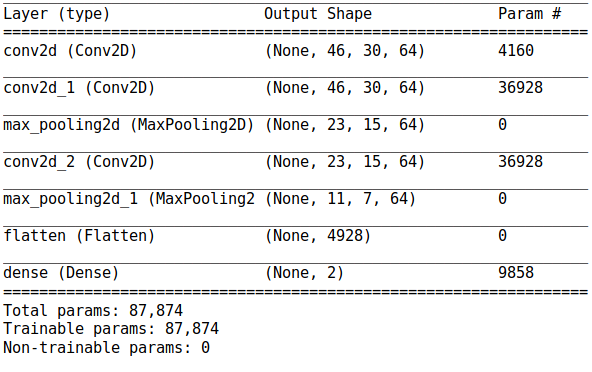
\includegraphics[width=11cm]{DL_architecture.png}
 		\caption{Arquitetura do modelo de \textit{Deep Learning} utilizado.}
 		\label{fig:DLArchUsed}
 	\end{figure}
 
 	O último valor do \textit{Shape} de cada camada é a quantidade de neurônios que ela possui, enquanto os demais valores são o número de linhas e colunas da imagem. O valor "4" que era de se esperar devido aos 4 filtros não aparece explicitamente na estrutura de arquitetura do modelo, todavia, é um comportamento normal visto que neste caso ele funciona como se fosse uma imagem em "RGBA" (uma matriz para veremlho, azul, verde e transparência).
 	
 	Em seguida, foi definida uma \textit{random seed} para poder fixar quaisquer tipos de aleatoriedades intrínsecas ao modelo. Assim, o mesmo foi treinado em 2,3,5 e 10 épocas (número este também baseado nos exemplos citados), obtendo um resultado satisfatório quando o valor foi de 10 épocas, pois sua acurácia foi mais alta e ainda assim não ficou "viciado".
 	
 	\section{Resultados e comparações}
	\newpage
  \chapter{Interpolação através de Processo Gaussiano}
  \label{chap:GP}
  
	\section{Escolha da Biblioteca}
		
	\section{Aleatoriedades e \textit{Random Seeds}}
			
	\section{\textit{Kernel Functions}}
			
	\section{Demais Observações}
			Valor negativo e Mean function, erro grande, melhor overfittado que underfitado
			
	\section{Resultados das Interpolações}
		
	\section{Identificação e Justificativa do Erro}
	\newpage 
  \chapter{Resultados e Discussões}
  \label{chap:Result}
	\newpage
  \chapter{Conclusões}
  \label{chap:Concl}
	\section{Conclusões Finais} 	  
		
			Falar que o Algoritmo de hoje já é bem robusto
		
	\section{Trabalhos Futuros} 
		
			Falar de consertar o Erro e pah
		  

  \backmatter
  \bibliographystyle{coppe-unsrt}
  \bibliography{bibliografia}

  \appendix
  \chapter{Repositório do Código}
  
  Todo o código desenvolvido encontra-se disponível no repositório público do \textit{GitHub}, a fim de poder ser desenvolvido e modificado por qualquer pessoa que deseje contribuir ou estudar este projeto, podendo ser acessado no seguinte link: \href{https://github.com/FelipeMFO/supernova_identification}{https://github.com/FelipeMFO/supernova\_identification}.
\end{document}
%% 
%%
%% End of file `example.tex'.
